\chapter{非平衡统计力学}

在前面的章节中我们主要研究了各种物理量统计平均值的计算问题,这些平均值以高精度表示出从对 \textcolor{RoyalBlue}{\textbf{\kaishu 处于平衡}} 的给定系统进行有关测量所预期得到的结果。但是,对于近平衡和原理平衡的体系,基于以下几方面的理由,能谱-配分函数-热力学量的研究范式就显得力不从心:

\begin{figure}[ht]
    \centering
    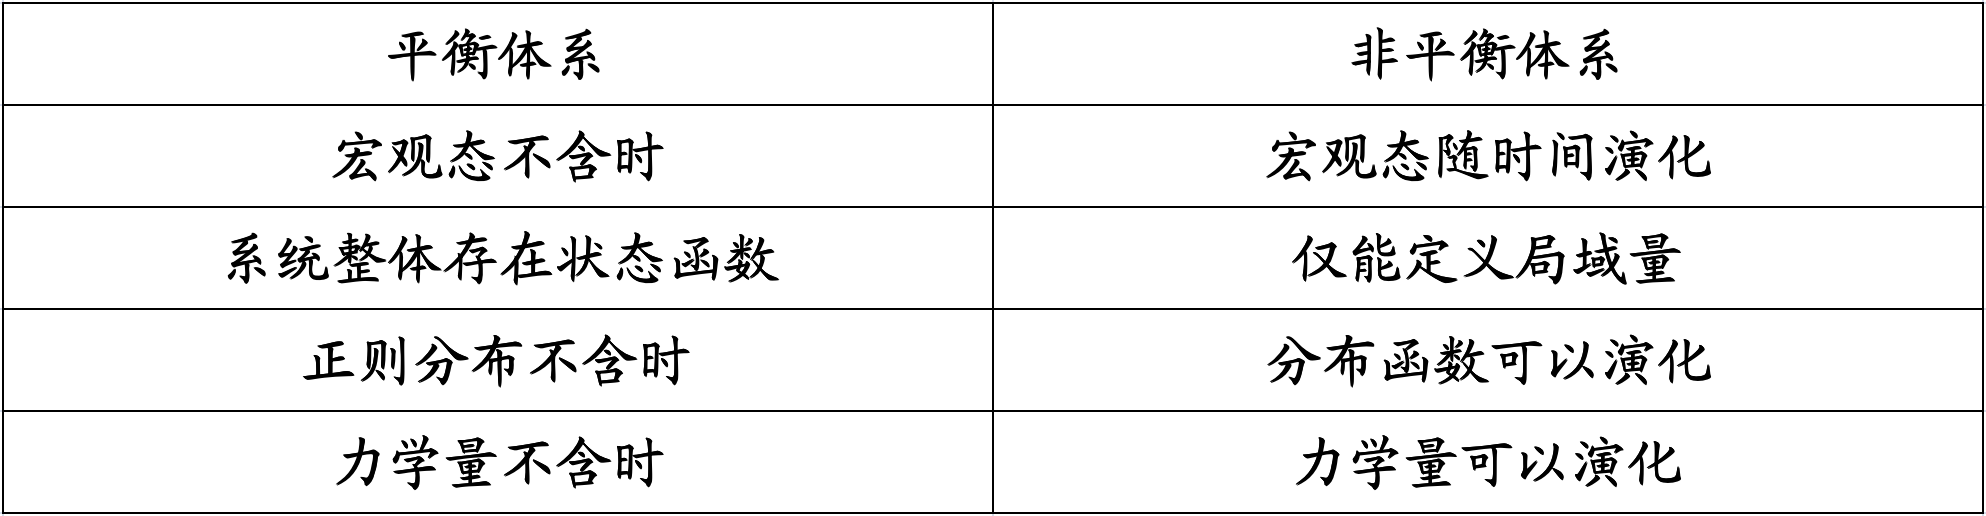
\includegraphics[width=1\textwidth]{figures/equ-nonequ.png}
    \caption{\kaishu 平衡态与非平衡态的区别}
    \label{fig:equ-nonequ}
\end{figure}

由此可见,对于非平衡系统, \textcolor{RoyalBlue}{\textbf{\kaishu 演化}} 二字是核心。本章将从两个方面来研究非平衡系统的演化:一是 \textcolor{RoyalBlue}{\textbf{\kaishu 分布的演化}},即如何从初始分布演化到平衡分布,也就是说一个不处于平衡态的分布函数如何最终逼近平衡分布,并继续维持平衡分布;二是 \textcolor{RoyalBlue}{\textbf{\kaishu 力学量的演化}},即力学量如何从初始状态演化到平衡态,这将涉及关联函数的概念。这两种视角分别相当于量子力学中的薛定谔绘景和海森堡绘景,为了看出这一点,我们必须再次将目光投向 \textcolor{RoyalBlue}{\textbf{\kaishu 刘维尔定理}} 。

\section{再论刘维尔定理}

对于一个不显含时的力学量 $A$,其演化方程为
\begin{equation}\label{equ:刘维尔定理,不显含时}
    \frac{\mathrm{d} A}{\mathrm{d} t} =  [A, H]
\end{equation}
为了将它写成更一般的微分方程形式,我们定义 \textcolor{RoyalBlue}{\textbf{\kaishu 刘维尔算符}} 为
\begin{equation}\label{equ:刘维尔算符}
    \mathcal{L}A \equiv [A, H]
\end{equation}
这样,\eqref{equ:刘维尔定理,不显含时} 就可以写成
\begin{equation}\label{equ:刘维尔定理,不显含时,微分方程形式}
    \frac{\mathrm{d} A}{\mathrm{d} t} =  \mathcal{L}A
\end{equation}
那么自然而然地,形式解
\begin{equation}\label{equ:形式解}
    A(\Gamma,t) = e^{t\mathcal{L}}A(\Gamma,0)
\end{equation}

代表点密度也是一个特殊的力学量,但由于刘维尔定理的存在,它的演化方程可以写成
\begin{equation}\label{equ:代表点密度的演化方程}
    f(\Gamma,t) =  e^{-t\mathcal{L}}f(\Gamma,0)
\end{equation}

同时,刘维尔算符具有反自伴性(Posson括号的微分性质导致的),即
\begin{align}\label{equ:反自伴性}
    \int (\mathcal{L}A)*B \,\mathrm{d}\Gamma= -\int A*(\mathcal{L}B) \,\mathrm{d}\Gamma \\
    \int (e^{t\mathcal{L}}A)*B \,\mathrm{d}\Gamma= \int A*(e^{t\mathcal{L}}B) \,\mathrm{d}\Gamma
\end{align}

有了刘维尔算符,我们就可以将力学量的系综平均写为较为简洁的形式。不过这样的平均有两种角度来看待: \textcolor{RoyalBlue}{\textbf{\kaishu 从薛定谔绘景的角度,力学量 $A$ 仅是相点位置的函数 $A(\Gamma)$ ,而占据这些相点的概率分布是随时间变化的}} ,因此力学量的系综平均可以写为
\begin{equation}\label{equ:力学量的系综平均,薛定谔绘景}
    \langle A(t) \rangle = \int A(\Gamma) f(\Gamma, t) \,\mathrm{d}\Gamma
\end{equation}
\textcolor{RoyalBlue}{\textbf{\kaishu 从海森堡绘景的角度,力学量 $A$ 是随时间变化的,而概率分布 $f$ 是相点位置的函数 $f(\Gamma)$ ,不随时间改变}} ,所以力学量的系综平均也可以写为
\begin{equation}\label{equ:力学量的系综平均,海森堡绘景}
    \langle A(t) \rangle = \int A(\Gamma,t) f(\Gamma) \,\mathrm{d}\Gamma
\end{equation}
这二者的联系可以通过如下方式说明:
\begin{align*}
    \int A(\Gamma) f(\Gamma, t) \,\mathrm{d}\Gamma = \int A(\Gamma) e^{-t\mathcal{L}}f(\Gamma,0) \,\mathrm{d}\Gamma \\
    = \int e^{t\mathcal{L}}A(\Gamma) f(\Gamma,0) \,\mathrm{d}\Gamma = \int A(\Gamma,t) f(\Gamma) \,\mathrm{d}\Gamma
\end{align*}
\begin{justification}{\kaishu 反思与质疑}
\kaishu \fontsize{11pt}{16pt}
    这里直接将依赖关系隐去可能会导致一定程度的困惑,但是必须牢记,我们观察对 $A(t)$ 所有实验可能值的平均值时, \textcolor{RoyalBlue}{\textbf{\kaishu  所抽取的样本来自初始条件的分布}},也就是说
    \[
        \langle A(t) \rangle = \int A(\Gamma_0\rightarrow \Gamma_t) f(\Gamma_0; \text{time} = 0) \,\mathrm{d}\Gamma_0 = \int A(\Gamma_0;\text{time} = 0) f(\Gamma_0,t) \,\mathrm{d}\Gamma_0
    \]
    前者是海森堡绘景,后者是薛定谔绘景,被积变量总是遍历整个相空间,所以 $\mathrm{d}\Gamma_0 = \mathrm{d}\Gamma$ 。
\end{justification}

此外,平衡分布是一个与系统哈密顿量对易的力学量:
\begin{equation}\label{equ:平衡分布和哈密顿量对易}
    f_{eq}(H) = \frac{e^{-\beta H}}{Z} ,\quad\mathcal{L}f_{eq}(H) = [f_{eq}(H), H] = 0
\end{equation}

所以,与平衡系统不同,对于非平衡系统我们有两种方式来求一个力学量的系综平均,即 \eqref{equ:力学量的系综平均,薛定谔绘景} 和 \eqref{equ:力学量的系综平均,海森堡绘景} 。运用前者,我们将从 \textcolor{RoyalBlue}{\textbf{\kaishu 布朗运动}} 开始,研究分布函数随时间的演化,导出其所满足的偏微分方程,即 \textcolor{RoyalBlue}{\textbf{\kaishu 福克尔-普朗克方程}} ;运用后者,我们将力学量视为随机过程,引入 \textcolor{RoyalBlue}{\textbf{\kaishu 关联函数}} ,建立其与 \textcolor{RoyalBlue}{\textbf{\kaishu 响应函数}} 的联系,研究 \textcolor{RoyalBlue}{\textbf{\kaishu 涨落耗散定理}} 。

\section{分布的演化:薛定谔绘景}

\subsection{布朗运动的爱因斯坦理论}

独立和,概率密度的推导以及使用斯特林公式后的渐进形式

引入扩散方程,指出扩散方程的解和这里相同,从而指出概率的微观解释与宏观解释的等价性将导致随机过程与扩散方程的等价性

\subsection{福克尔-普朗克方程}

抄 pathria

\section{力学量的演化:海森堡绘景}


\subsection{关联函数及其稳态性质}

抄笔记

\subsection{布朗运动的朗之万理论}

抄pathria,给出唯像的朗之万方程、爱因斯坦关系,并指出爱因斯坦关系是涨落耗散定理的一种表述形式

\section{线性响应与涨落耗散定理}

\subsection{昂萨格回归假说}

首先从回归假说的神秘性开始,即自然涨落和弛豫不可分辨,抄一点chandler,指出在扩散中的应用。

\subsection{静态响应与静态弛豫}

研究静态弛豫,证明假说的正确性,抄笔记

\subsection{响应函数}

一般情况的弛豫——定义响应函数,物理意义、因果性、稳态性,抄笔记

指出响应函数与关联函数的关系,这就是涨落耗散定理

\subsection{从线性响应理论到朗之万方程}

三个关键认识
